\chapter{Handleiding voor ontwikkelaars}
\label{appendix-g}

Deze handleiding is bedoeld voor mensen die de code van synchronisatiebibliotheek of de Max/MSP modules willen analyseren of wijzigen. Het volledige project is openbaar beschikbaar op \url{https://github.com/wardva/SignalSync}. Het Java-project bevindt zich in de map \textbf{SignalSync}.

\section*{Project importeren in Eclipse}

Na het binnenhalen van het project kan de map \textbf{SignalSync} geïmporteerd worden in Eclipse. Maak hiervoor een nieuw Java project aan en wijzig de \textit{default location} in het pad van \textbf{SignalSync}. Na het importeren zullen enkele foutmeldingen te zien zijn wegens gebroken afhankelijkheden. 

Het project is afhankelijk van volgende softwarebibliotheken: TarsosDSP, Panako en TeensyDAQ. De TarsosDSP broncode kan gedownload worden van \url{https://github.com/JorenSix/TarsosDSP}, de Panako broncode van \url{http://panako.be/releases/Panako-latest/readme.html} en de TeensyDAQ broncode van \url{https://github.com/JorenSix/TeensyDAQ}. 

Na het importeren van deze projecten in eclipse en het instellen van de projecten als \textit{reference project} moeten er nog enkele JAR bestanden worden toegevoegd. 
\newpage
\textbf{jssc-2.7.0.jar}, deze bibliotheek is te downloaden van: \url{https://code.google.com/archive/p/java-simple-serial-connector/downloads}.

\textbf{max.jar}, deze bibliotheek bevindt zich in de Max/MSP installatiemap standaard onder Windows: \texttt{C:\textbackslash Program Files\textbackslash Cycling '74\textbackslash Max 7\textbackslash resources\textbackslash packages\textbackslash max-mxj\textbackslash \\ java-classes\textbackslash lib}

Na het toevoegen van de \textit{references} en JAR bestanden zouden de foutmeldingen moeten verdwijnen.

\section*{Het project koppelen aan Max/MSP}

Het zou vrij omslachtig zijn om telkens een JAR bestand te moeten genereren vooraleer een bepaalde module in Max/MSP uitgetest kan worden. Daarom is het ook mogelijk om Max/MSP te koppelen aan een map met classfiles. Hiervoor moet het configuratiebestand \texttt{max.java.config.txt} uit de Max/MSP installatiemap worden aangepast. Onder Windows bevindt het bestand zich standaard in volgende map: \texttt{C:\textbackslash Program Files\textbackslash Cycling '74\textbackslash Max 7\textbackslash resources\textbackslash packages\textbackslash max-mxj\textbackslash java-classes}.

Met volgende lijn wordt er verwezen naar een map met classfiles: \texttt{max.dynamic.class.dir <<pad>>}. Hierbij moet \texttt{<<pad>>} worden vervangen door het pad van de map (backslashes escapen met een backslash). Er moet ook naar elke afhankelijkheid verwezen worden. Verwijs dus ook naar de map met classfiles van TarsosDSP en Panako. Ten slotte moet ook de jSSC JAR worden opgenomen in het bestand. Voeg daarom volgende lijn toe waarbij \texttt{<<pad>>} staat voor de map waarin zich de JAR bevindt: \texttt{max.dynamic.jar.dir <<pad>>}.

\section*{Debuggen van Max/MSP modules}

Het is mogelijk om de broncode in Eclipse te debuggen terwijl een module in Max/MSP wordt uitgevoerd. Deze handige feature vereist wel wat configuratie.

Ten eerste moeten volgende lijnen aan het Max/MSP configuratiebestand (zie vorige sectie) worden toegevoegd:

\begin{allintypewriter}
max.jvm.option -Xdebug \\
max.jvm.option -Xnoagent \\
max.jvm.option -Xrunjdwp:transport=dt\_socket\textbackslash ,address=8074\textbackslash,server=y\textbackslash,suspend=n \\
max.jvm.option -XX:-UseSharedSpaces
\end{allintypewriter}
Het is mogelijk dat deze lijnen in het standaard configuratiebestand in commentaar staan. Indien dit het geval zou zijn dan is het voldoende om de puntkomma's voor en achter de regel te verwijderen.

\begin{figure}[!tbph]
	\centering
	\subfloat{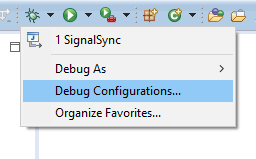
\includegraphics[width=0.3\textwidth]{debugconf.png}}
	\hfill
	\subfloat{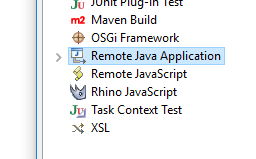
\includegraphics[width=0.3\textwidth]{debugremote.png}}
	\hfill
	\subfloat{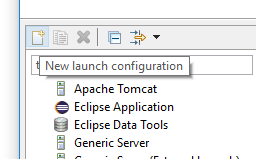
\includegraphics[width=0.3\textwidth]{debugnew.png}}
	\captionsetup{width=0.7\textwidth}
	\caption{Nieuwe debug configuration aanmaken in Eclipse}
	\label{debugconf}
\end{figure}

Ga hierna naar \textbf{Debug Configurations} in Eclipse. Selecteer \textbf{Remote Java Application} en klik vervolgens op het icoon van \textbf{new launch configuration}. Deze stappen worden verduidelijkt in figuur \ref{debugconf}.

\begin{figure}[!tbph]
	\captionsetup{width=0.7\textwidth}
	\caption{De debug configuratie in Eclipse}
	\begin{center}
		\advance\parskip0.3cm
		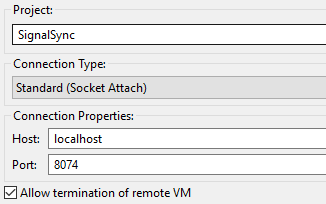
\includegraphics[width=0.5\textwidth]{debugsettings.png}
	\end{center}
	
	\label{debugsettings}
\end{figure}

Geef vervolgens de configuratie een naam en blader bij \textbf{Project} naar het te debuggen project (SignalSync). Kies bij \textbf{Connection Type} voor \textbf{Standard (Socket Attach)}. Bij \textbf{Connection Properties} moet de poort worden opgegeven die in het Max/MSP configuratiebestand gespecificeerd is (standaard 8074). Aangezien de applicatie lokaal draait moet bij \textbf{Host} \texttt{localhost} of \texttt{127.0.0.1} worden opgegeven. Met \textbf{Allow termination of remote VM} kan worden ingesteld of de Max/MSP VM vanuit Eclipse mag worden afgesloten. Figuur \ref{debugsettings} toont een screenshot van de instellingen.

Het debuggen wordt gestart door eerst de Max/MSP patch te openen en vervolgens het debuggen in Eclipse te starten met de zojuist aangemaakt debug configuratie. Bij het starten van de patch is het nu mogelijk om via breakpoints door de code navigeren.

\section*{Genereren van testdata}

De bestanden die vereist zijn voor het uitvoeren van de testen bevinden zich niet in het GitHub repository maar moeten nog gegenereerd worden. 

De eerste stap voor het genereren van de bestanden is het uitvoeren van het perl-script \texttt{TestSetGenerator.pl}. Dit script kan gedownload worden van de map \textbf{Scripts} in het GitHub repository. Het script maakt van een groep mp3-bestanden verschillende varianten aan (zie \ref{latency-test} en \ref{sine-test}). In het script moet de bron- en doelmap worden opgegeven.

Met behulp van de Java applicatie \texttt{SlicerApp} uit de package \texttt{be.signalsync.app} kunnen de gegenereerde bestanden worden omgezet in slices. Deze slices dienen als input voor enkele testen.


